\begin{enumerate}[label=\thechapter.\arabic*,ref=\thechapter.\theenumi]

\item Consider the discrete time signal $x\sbrak{n} = u\sbrak{-n+5} - u\sbrak{n+3}$, where
\[u\sbrak{n} = 
\begin{cases}
    1;n\geq0\\
    0;n<0
\end{cases}
\]
The smallest n for which $x\sbrak{n} = 0$ is?
\\ \solution
\iffalse
\let\negmedspace\undefined
\let\negthickspace\undefined
\documentclass[journal,12pt,twocolumn]{IEEEtran}
\usepackage{cite}
\usepackage{amsmath,amssymb,amsfonts,amsthm}
\usepackage{algorithmic}
\usepackage{graphicx}
\usepackage{textcomp}
\usepackage{xcolor}
\usepackage{txfonts}
\usepackage{listings}
\usepackage{enumitem}
\usepackage{mathtools}
\usepackage{gensymb}
\usepackage{comment}
\usepackage[breaklinks=true]{hyperref}
\usepackage{tkz-euclide} 
\usepackage{listings}
\usepackage{gvv}                                        
\def\inputGnumericTable{}                                 
\usepackage[latin1]{inputenc}                                
\usepackage{color}                                            
\newtheorem{theorem}{Theorem}[section]
\usepackage{array}                                            
\usepackage{longtable}                                       
\usepackage{calc}                                             
\usepackage{multirow}                                         
\usepackage{hhline}                                           
\usepackage{ifthen}                                           
\usepackage{lscape}
\newtheorem{problem}{Problem}
\newtheorem{proposition}{Proposition}[section]
\newtheorem{lemma}{Lemma}[section]
\newtheorem{corollary}[theorem]{Corollary}
\newtheorem{example}{Example}[section]
\newtheorem{definition}[problem]{Definition}
\newcommand{\BEQA}{\begin{eqnarray}}
\newcommand{\EEQA}{\end{eqnarray}}
\newcommand{\define}{\stackrel{\triangle}{=}}
\theoremstyle{remark}
\newtheorem{rem}{Remark}
\begin{document}
\bibliographystyle{IEEEtran}
\vspace{3cm}
\title{GATE: IN/28}
\author{EE23BTECH11040 - Manoj Kumar Ambatipudi$^{*}$% <-this % stops a space
}
\maketitle
\newpage
\bigskip
\renewcommand{\thefigure}{\theenumi}
\renewcommand{\thetable}{\theenumi}
\textbf{QUESTION:}
Consider the discrete time signal $x\sbrak{n} = u\sbrak{-n+5} - u\sbrak{n+3}$, where
\[u\sbrak{n} = 
\begin{cases}
    1;n\geq0\\
    0;n<0
\end{cases}
\]
The smallest n for which $x\sbrak{n} = 0$ is?\\
\textbf{Solution:}
\fi
From \figref{IN/28/fig1}, the minimum value of $n$ is given as 
\begin{align}
    n = -3
\end{align}
\begin{figure}[h!]
\renewcommand\thefigure{1}
    \centering
    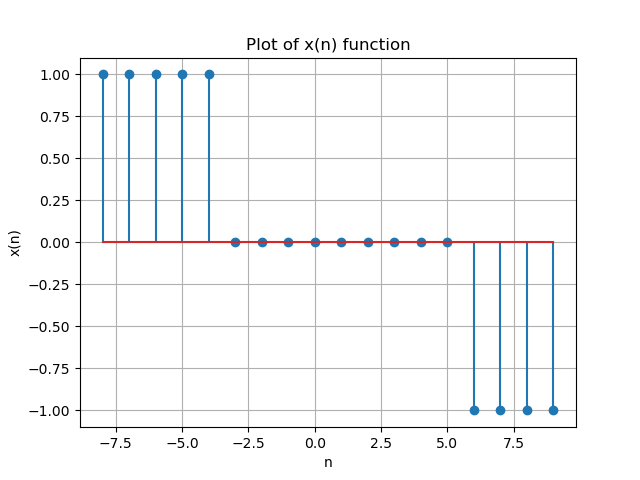
\includegraphics[width=1.0\columnwidth]{2023/IN/28/figs/fig_1.png}
    \caption{Plot of function $x\brak{n}$ taken from python3}
    \label{IN/28/fig1}
\end{figure}


\newpage
\item Two sequences $x_1\sbrak{n} $ and $ x_2 \sbrak{n}$ are described as follows:
\begin{align}
x_1\sbrak{0} = x_2\sbrak{0} = 1\\
x_1\sbrak{1} = x_2\sbrak{2} = 2\\
x_1\sbrak{2} = x_2\sbrak{1} = 1
\end{align}
$x_1\sbrak{n} = x_2\sbrak{n} = 0$ for all $n<0$ and $n>2$\\
\\
If $x\sbrak{n}$ is obtained by convoluting $x_1\sbrak{n}$ with $x_2\sbrak{n}$, which of the following equations is/are TRUE?\\
\\
(A) $x\sbrak{2} = x\sbrak{3}$\\
\\
(B) $x\sbrak{1} = 2$\\
\\
(C) $x\sbrak{4} = 3$\\
\\
(D) $x\sbrak{2} = 5$\\

\solution
\pagebreak
\item A series \brak{S} is given as S=1+3+5+7+9+..... The sum of the first 50 terms of S is \underline{\hspace{1in}}
\solution
\pagebreak
\end{enumerate}
